%!TEX root = ../documentation.tex

\chapter{Evaluation}\label{cha:evaluation}

The previous chapter provides all the information needed to evaluate whether a generalized shell application is needed and how it would look like.
In the following the experts opinion on this question is presented, which concludes the experts input to this thesis.
Afterwards, one practical example for each scenario from \ref{cha:scenarios_types} is shown.
This will be used to evaluate if the most mentioned framework from the experts can fulfill all the needs outlined in the chapter \ref{cha:requirement}.





\section{Expert opinions}\label{cha:evaluation_experts}

The final question of the expert interviews was the thesis question, \ref{cha:appendix_expertinterview_questions}.
It is, whether a generalized shell application is needed or not.
All experts believe, that something is needed, but some are more precise of what is actually needed.
One framework was mentioned by \textciteRehm{}, \textciteMezzalira{}, \textciteJovanovic{} and \textciteSteyer{}, namely \textit{Single-SPA}.
This is the most known \ac{MF} framework.
They believe, that it is at least a step into the right direction in fulfilling the need of a generalized shell application.

\textit{Single-SPA} is a meta framework, which means it manages other frameworks (more information is provided in the section \ref{cha:evaluation_singlespa}).
\citeauthorMezzalira{} points out, that he believes the approach they have built for DAZN is slightly more flexible than \textit{Single-SPA}.
Still, if he had known of \textit{Single-SPA} 3 years ago, he would have used it.

Besides this one practical approach, \textciteHuber{} points out that \ac{MFA} is still new, which is why no clear answer is available yet.
This is confirmed by \textciteJovanovic{} and \textciteOlleck{}.
\citeauthorJovanovic{} believes that an example application that can be customized for other projects would be great.
Such an application can be used as a showcase for new customers and as base for new projects.
As a result, this lowers the barrier to getting started with the \ac{MFA}.
On the other hand, \citeauthorOlleck{} thinks that an example is not enough and instead standards are needed.
These standards would allow to mitigate problems which all projects will face at some point.
This could include for example, how to manage shared state or how to handle intercommunication.
However, he points out, that not everything can be standardized, because there are custom needs for each shell implementation as well.
Therefore, \citeauthorOlleck{} and also \citeauthorSteyer{} believe, that a shell framework is needed instead of a generalized shell application.

To sum up, the framework \textit{Single-SPA} was mentioned by almost all experts which also believe it could fulfill the need.
This will be evaluated in section \ref{cha:evaluation_singlespa}.
In general all experts agree on the idea that some form of generalized shell is needed.





\section{Application examples}\label{cha:evaluation_example}

Before evaluating \textit{Single-SPA}, it is important to outline what actual applications look like in terms of approaches.
This helps to set goals, which \textit{Single-SPA} needs to achieve in order to pass as general shell application.
The example applications are meant to cover a wide range of requirement combinations and still fit into the named scenarios from \ref{cha:scenarios_types}.
Hence, the facts named in section \ref{cha:scenarios_types} are used to determine which requirements are needed.
From these facts, only integration requirements can be extracted from them.
The structure of this section is, that the examples are explained, then some common facts are outlined and finally the assessment based on \ref{cha:requirements_conclusion_assessment} is conducted.



\paragraph{\nameref{cha:scenarios_enterprise} (EA)}\label{cha:evaluation_enterprise}

Before describing the enterprise application example, it helps to first outline what the differences are to other application types in regards to integration requirements.
An \nameref{cha:scenarios_enterprise} has no need for the \nameref{cha:requirement_detail_integration_crawler} requirement, because it is typically developed in-house and therefore no search engine needs to index the application.
Another needless requirement is \nameref{cha:requirement_detail_integration_abstraction}, because such an application is typically not used from a game console or smart TV.
The same applies for the \nameref{cha:requirement_detail_integration_extensible} requirement, because the application must be used by multiple companies so that extensions are created.
On the other hand, it is possible that a \ac{MF} is reused in multiple applications and therefore the \nameref{cha:requirement_detail_integration_interoperable} requirement could be needed.

After outlining the general integration requirement needs for an \nameref{cha:scenarios_enterprise}, an example enterprise application is shown to better emphasize the theoretical information.
This enterprise application example is mainly based on the application described by \textciteOlleck{}.
Its only difference is, that the \nameref{cha:requirement_detail_integration_lifecycle} requirement is not part of the application.
Based on the other experts inputs, there is no need for this requirement, if the target device is performant.
Also, this reduces the complexity for the shell and keeps the state of each \ac{MF}.

In case of page composition, both \nameref{cha:requirement_detail_integration_widget} and \nameref{cha:requirement_detail_integration_pagelayout} requirements are part of the example application.
The first is needed for cross cutting concern \ac{UI} elements and the latter only is needed for a tile-based arrangement.
Another requirement that can effect page composition, is part of this example, which is \nameref{cha:requirement_detail_integration_sharedlogic}.
It is needed to share the navigation bar and provide a shared toast feature.
Finally, in terms of the \nameref{cha:requirement_detail_state_exchange} requirement, a Redux store is selected, because of its superior bug fixing feature.

This concludes the \nameref{cha:scenarios_enterprise} example, because no more information would change the outcome of the quadrant chart described in \ref{cha:requirements_conclusion_assessment} and all integration requirements are considered.



\paragraph{\nameref{cha:scenarios_consumer} (CA)}\label{cha:evaluation_consumer}

Before describing the example, it helps to first outline what the differences are to other application types in regards to integration requirements.
While the \nameref{cha:requirement_detail_integration_crawler} requirement is not needed for a \nameref{cha:scenarios_enterprise}, it is certainly a relevant feature for a \nameref{cha:scenarios_consumer}.
However, its importance varies:
For example, an e-commerce shop needs the requirement, while a banking application could be fine without it.
Another requirement which is needed is \nameref{cha:requirement_detail_integration_abstraction}, as outlined by \textciteMezzalira{}.
In his example, the application DAZN needs to work in game console and smart TV browsers.
A probably rare requirement is \nameref{cha:requirement_detail_integration_extensible}.
For this \textciteSteyer{} provided the example, that gaming or gambling applications sometimes include third party applications via iFrames.
Hence, it is relevant for a \nameref{cha:scenarios_consumer}.
On the other hand, it is unlikely that a \ac{MF} is needed in multiple applications.
As a result, \nameref{cha:requirement_detail_integration_interoperable} is left out.

Similarly to the previous scenario, an example application is presented as well.
This example is mainly based on the application described by \textciteMezzalira{}.
The example application has two differences compared to the described application by \citeauthorMezzalira{}.
First, it includes the \nameref{cha:requirement_detail_integration_widget} requirement to allow for cross cutting \acp{UI} and second the \nameref{cha:requirement_detail_integration_sharedlogic} requirement is added to share the navigation panel.

The scenario application from \textciteMezzalira{} also uses the \nameref{cha:requirement_detail_integration_lifecycle} requirement to dereference unused \acp{MF}.
Moreover, because there is no need for multiple \acp{MF} per page, the \nameref{cha:requirement_detail_integration_pagelayout} requirement is not part of the example application.
Another aspect was already explained in the beginning, which is the \nameref{cha:requirement_detail_integration_abstraction} requirement.
This is part of the example, because it should work on consoles and smart TV browsers as well.
Finally, for the \nameref{cha:requirement_detail_state_exchange} requirement the shell is responsible to cache \ac{API} fetches to reduce duplicate requests.



\paragraph{\nameref{cha:scenarios_offshelf} (OA)}\label{cha:evaluation_offshelf}

Finally, there is the \nameref{cha:scenarios_offshelf}.
It is essentially a mix of \nameref{cha:scenarios_enterprise}s and \nameref{cha:scenarios_consumer}s, which was outlined in \ref{cha:scenarios_types}.
Also, only \textcite{Grijzen.2019} provided information about this application type, which does not allow to generalize it.
Therefore, the application he describes is used as the example application.

\textcite{Grijzen.2019} describes an application that monitors other applications.
The application needs a flexible layout, thus the \nameref{cha:requirement_detail_integration_pagelayout} requirement is needed.
But they do not need the \nameref{cha:requirement_detail_integration_widget} requirement.
Another requirement that is not needed is the \nameref{cha:requirement_detail_integration_abstraction}.

A priority for the application is performance, which is why code and data is shared as much as possible.
As a result, only one version of React is used and common dependencies are shared.
In the application a library is used to cache fetch data from an endpoint.
Hence, fetch data is cached, but the complexity is not within the shell.
Another aspect which accounts into sharing is the \nameref{cha:requirement_detail_integration_sharedlogic} requirement.
In case of the application \citeauthor{Grijzen.2019} describes that the navigation panel is part of the shell and is dynamically rendered.
Furthermore, a platform \ac{API} is shared over the shell with all \acp{MF} for common actions.
Finally, the \nameref{cha:requirement_detail_integration_lifecycle} requirement was not mentioned by him.
Because the other requirements heavily favor performance, it can be suspected, that it is part of the application.

% requirements:
% \xmark{} \nameref{cha:requirement_detail_integration_crawler}, because the app is not public (its a monitoring tool)
% \cmark{} \nameref{cha:requirement_detail_integration_interoperable}, was main goal
% \xmark{} \nameref{cha:requirement_detail_integration_abstraction}, no need to run on consoles or smart TVs
% \cmark{} \nameref{cha:requirement_detail_integration_extensible}



\paragraph{Common facts}

\begin{table}
    \begin{tabular}{|l|cc|cc|}
        \multirow{2}{*}{\textbf{Requirement}}                                  &
        \multicolumn{2}{c|}{\textbf{\hyperref[cha:evaluation_enterprise]{EA}}} &
        \multicolumn{2}{c|}{\textbf{\hyperref[cha:evaluation_consumer]{CA}}}
        \\
                                                                               &
        \multicolumn{1}{c|}{mandatory}                                         &
        optional                                                               &
        \multicolumn{1}{c|}{mandatory}                                         &
        optional
        \\ \hline
        \nameref{cha:requirement_detail_integration_loading}                   & \cmark{} &          & \cmark{} &          \\
        \nameref{cha:requirement_detail_integration_lifecycle}                 &          & \cmark{} & \cmark{} &          \\
        \nameref{cha:requirement_detail_integration_routing}                   & \cmark{} &          & \cmark{} &          \\
        \nameref{cha:requirement_detail_integration_configuration}             & \cmark{} &          & \cmark{} &          \\
        \nameref{cha:requirement_detail_integration_integration}               & \cmark{} &          & \cmark{} &          \\
        \nameref{cha:requirement_detail_integration_crawler}                   &          &          &          & \cmark{} \\
        \nameref{cha:requirement_detail_integration_sharedlogic}               &          & \cmark{} &          & \cmark{} \\
        \nameref{cha:requirement_detail_integration_widget}                    &          & \cmark{} &          & \cmark{} \\
        \nameref{cha:requirement_detail_integration_pagelayout}                &          & \cmark{} &          & \cmark{} \\
        \nameref{cha:requirement_detail_integration_interoperable}             &          & \cmark{} &          &          \\
        \nameref{cha:requirement_detail_integration_abstraction}               &          &          &          & \cmark{} \\
        \nameref{cha:requirement_detail_integration_extensible}                &          &          &          & \cmark{}
    \end{tabular}
    \centering
    \caption{Overview of integration requirement distribution between \nameref{cha:scenarios_enterprise}s and \nameref{cha:scenarios_consumer}s}
    \label{tbl:evaluation_requirement_distribution}
\end{table}

While defining the example applications based on the experts inputs, there are some facts that became apparent, which need to be outlined.
The first fact was hinted in the examples, which is that there are some similarities between the example application requirements.
Table \ref{tbl:evaluation_requirement_distribution} shows which integration requirements are needed or optional for the \nameref{cha:scenarios_enterprise} and \nameref{cha:scenarios_consumer}, based on the examples.
Also, because the \nameref{cha:scenarios_offshelf} is a mix of the other two, it is not included in the Table.
Abbreviations for the application type names are applied in the Table, which are \nameref{cha:scenarios_enterprise} is \textit{EA}, \nameref{cha:scenarios_consumer} is \textit{CA} and \nameref{cha:scenarios_offshelf} is \textit{OA}.

The Table \ref{tbl:evaluation_requirement_distribution} visualizes two findings.
The first is that the requirements \nameref{cha:requirement_detail_integration_loading}, \nameref{cha:requirement_detail_integration_routing}, \nameref{cha:requirement_detail_integration_configuration} and \nameref{cha:requirement_detail_integration_integration} are always needed.
This is in line with the experts statements for the interview question five, which determines critical requirements for a shell application.
An overview of which requirement was mentioned for what question, is shown in Table \ref{tbl:adx_requirements_references}.
The only outlier in regards to the interview question five answers, is the \nameref{cha:requirement_detail_integration_lifecycle} requirement.
This requirement is considered critical by \textciteRehm{}, but not universally needed.
It is rather only needed for performance oriented applications.

The second finding is, that \nameref{cha:requirement_detail_integration_widget}, \nameref{cha:requirement_detail_integration_pagelayout} and \nameref{cha:requirement_detail_integration_sharedlogic} are optional in both cases.
The first two requirements mainly address page composition (see \ref{cha:theroy_extensions_composition}) whereas the last is about sharing \ac{UI} or common business functions.
All three requirements are important for the general structure of the application, but they are optional.



\paragraph{Assessment}

\begin{table}
    \setlength{\tabcolsep}{5pt} % Default value: 6pt
    \begin{tabular}{|c|l|cc|cc|cc|}
        \multicolumn{2}{|c|}{\textbf{Requirements}}                                    &
        \multicolumn{2}{c|}{\textbf{\hyperref[cha:evaluation_enterprise]{EA}}}         &
        \multicolumn{2}{c|}{\textbf{\hyperref[cha:evaluation_consumer]{CA}}}           &
        \multicolumn{2}{c|}{\textbf{\hyperref[cha:evaluation_offshelf]{OA}}}
        \\
        Shell                                                                          &
        \multicolumn{1}{c|}{Application (App)}                                         &
        \multicolumn{1}{c|}{Shell}                                                     &
        App                                                                            &
        \multicolumn{1}{c|}{Shell}                                                     &
        App                                                                            &
        \multicolumn{1}{c|}{Shell}                                                     &
        App
        \\ \hline
        \multicolumn{2}{|c|}{\nameref{cha:requirement_detail_integration_pagelayout}}  &
        1                                                                              & 0          & 0          & 1          & 1          & 0                       \\
        \multicolumn{2}{|c|}{\nameref{cha:requirement_detail_integration_widget}}      &
        1                                                                              & 1          & 1          & 1          & 0          & 0                       \\
        \multicolumn{2}{|c|}{\nameref{cha:requirement_detail_integration_abstraction}} &
        0                                                                              & 0          & 1          & 1          & 0          & 0                       \\
        \multicolumn{2}{|c|}{\nameref{cha:requirement_detail_state_exchange}}          &
        0                                                                              & 2          & 2          & 1          & 1          & 0                       \\
        \multicolumn{2}{|c|}{\nameref{cha:requirement_detail_integration_sharedlogic}} &
        2                                                                              & 2          & 1          & 1          & 2          & 2                       \\
        \multicolumn{1}{|l|}{\nameref{cha:requirement_detail_integration_lifecycle}}   &
        \makecell[l]{\hyperref[cha:requirement_detail_performance]{Performance}                                                                                      \\(shared dependencies)} &
        0                                                                              & 0          & 1          & 1          & 1          & 2                       \\
        \multicolumn{1}{|l|}{- }                                                       &
        \makecell[l]{\hyperref[cha:requirement_detail_performance]{Performance}                                                                                      \\(shared core)} &
        -                                                                              & 0          & -          & 2          & -          & 2                       \\ \hline
        \multicolumn{2}{|r|}{\textbf{Sum}}                                             & \textbf{4} & \textbf{5} & \textbf{6} & \textbf{8} & \textbf{5} & \textbf{6}
    \end{tabular}
    \centering
    \caption{Example application evaluation result scores}
    \label{tbl:eval_app_scores}
\end{table}

\begin{figure}
    \centering
    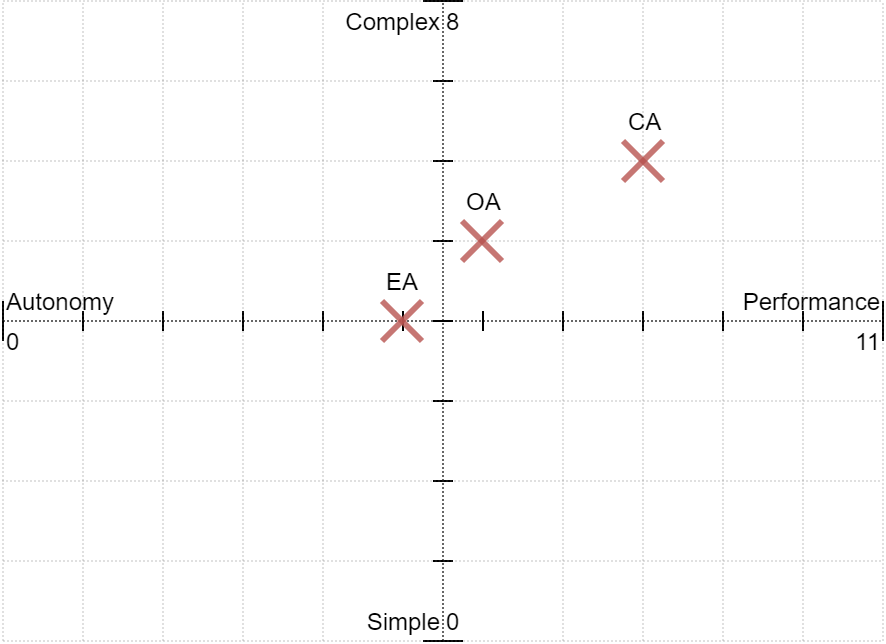
\includegraphics[scale=0.5]{quadrant_chart_filled.png}
    \caption{Quadrant chart from \ref{img:quadrant_chart} filled with evaluation results of the example applications}
    \label{img:quadrant_chart_filled}
\end{figure}


The named example applications are assessed, based on the score metric of section \ref{cha:requirements_conclusion_assessment}.
The evaluation result is shown in Table \ref{tbl:evaluation_requirement_distribution} and visualized in Figure \ref{img:quadrant_chart_filled}.
These examples satisfy the conceptual need for example applications, mentioned by \textciteJovanovic{}, which only leaves the need for an actual implementation.
An interesting fact shown in the Figure \ref{img:quadrant_chart_filled} is, that there seems to be a connection between the shell complexity and application performance.




\section{Existing solution Single-SPA}\label{cha:evaluation_singlespa}

The final part of this thesis is to evaluate, whether or not an existing framework fulfills all needs.
The framework in question is \textit{Single-SPA}, because it was mentioned by four of the six experts, which are namely \textciteRehm{}, \textciteMezzalira{}, \textciteJovanovic{} and \textciteSteyer{}.
There are two main things, which are evaluated.
The first is to check which requirements can be satisfied and secondly if \textit{Single-SPA} could be used to realize the example applications.

Based on the \textit{Single-SPA} documentation \cite{singlespa.2020}, all requirements and examples are feasible.
But there are some important aspects, which need to be outlined.
First and foremost, it fully depends on SystemJS.
SystemJS is a polyfill for \ac{ES}6 features that are not yet supported in browsers\footnotemark.
\footnotetext{\url{https://github.com/systemjs/systemjs} (Visited on 08/13/2020)}
It allows using a feature called \textit{Import Maps}.
Usually an import statement needs a \ac{URL} in the browser, but this browser specification allows to define an alias instead.
As a result, all \ac{JS} import statements can use the alias and the \ac{URL} is only set once in the \textit{Import Map}\footnotemark.
\footnotetext{\url{https://exploringjs.com/es6/ch_modules.html} (Visited on 08/13/2020)}

SystemJS supports this feature by providing a module loader implementation, which must be used instead of the native import statement.
Hence, all dependencies need to be transpiled into the SystemJS format in order to be used at all.
The transpilation can be handled by Webpack for instance.
While it adds some overhead, it allows to directly import code instead of providing it over a global variable.

Another aspect that is needed to implement many requirements is the shared Utility feature of \textit{Single-SPA} \cite{singlespa.2020}.
The \textit{Single-SPA} shell only provides features for the requirements \nameref{cha:requirement_detail_integration_loading}, \nameref{cha:requirement_detail_integration_lifecycle}, \nameref{cha:requirement_detail_integration_routing}, \nameref{cha:requirement_detail_integration} and \nameref{cha:requirement_detail_integration_widget}.
Other features are not provided out of the box, but can be realized with sharing Utility functions.
This addresses the \nameref{cha:requirement_detail_integration_abstraction}, \nameref{cha:requirement_detail_integration_sharedlogic}, \nameref{cha:requirement_detail_state_exchange},  \nameref{cha:requirement_detail_state_intercommunication} and \nameref{cha:requirement_detail_state_security} requirements, as well as styles from the \hyperref[cha:requirement_detail_style]{Consistent style} requirement.
This leaves the complexity out of the shell, while each project needs to implement it on its own.

The \nameref{cha:requirement_detail_integration_configuration} requirement is restricted in its flexibility.
Adding \acp{MF} is only possible via \ac{JS} code.
As a result, the \nameref{cha:requirement_detail_integration_extensible} requirement is possible, but it must be added via \ac{JS} code.
The final aspect for the requirements is, that the \textit{Single-SPA} feature which allows for the \nameref{cha:requirement_detail_integration_pagelayout} requirement is currently in a beta phase.
The feature is called Layout Engine \cite{singlespa.2020}.

While evaluating if the examples are theoretically feasible, there are three additional aspects that came up.
First, a Redux Store for the \hyperref[cha:evaluation_enterprise]{\nameref{cha:scenarios_enterprise}} example can be used in combination with \textit{Single-SPA}, although the team of \textit{Single-SPA} does not recommended using a global Redux store in general.
Next up is the caching approach for the \hyperref[cha:evaluation_consumer]{\nameref{cha:scenarios_consumer}} example.
This can be realized via a shared Utility function.
And finally, any shared dependencies or shared framework cores are distributed via SystemJS.


Ultimately \textit{Single-SPA} can achieve everything needed for a \ac{MF} application.
There are also two additional statements from the experts to it.
\textciteSteyer{} points out, that a \textit{Single-SPA} \ac{MF} can not be loaded in standalone mode.
This is a feature he demands, that \textit{Single-SPA} currently lacks.
The second statement is from \textciteMezzalira{} who states that \textit{Single-SPA} has a \enquote{opinionated} way of implementing \acp{MF}.
He did not further specify what he exactly means, but this may be that loading and importing is handled by SystemJS.

